\documentclass[12pt,openany,a4paper]{book}

\usepackage[T1]{fontenc}
\usepackage[utf8]{inputenc}
\usepackage{lmodern}
\usepackage[margin=2.5cm]{geometry}
\usepackage{setspace}
\usepackage{parskip}
\usepackage{microtype}

\usepackage{graphicx}
\usepackage{float}
\usepackage{array}
\usepackage{multirow}
\usepackage{makecell}

\setstretch{1.15}
\setlength{\emergencystretch}{3em}

\usepackage{amsmath}
\usepackage{amssymb}

\usepackage[numbers,sort&compress]{natbib}
\usepackage{url}
\DeclareUrlCommand\doi{\urlstyle{rm}}

\newcommand{\rotatedheading}[1]{%
  \rotatebox[origin=c]{90}{%
    \makebox[4.7cm][l]{#1}%
  }%
}

\begin{document}
\frontmatter
\begin{titlepage}
\renewcommand{\baselinestretch}{1.0}
\begin{center}
\vspace*{35mm}
\Huge\bf

        \begin{figure}[htpb]
            \centering
            
\includegraphics[width=0.6\linewidth]{UQ_Logo.png}
        \end{figure}

        \vspace*{25mm}

        Privacy-Preserving Federated Learning\\
        for Distributed Skin Disease Classification\\
\vspace{20mm}
\large\sl
		by\\
		ALEX GU
		\medskip\\
\rm
		School of Electrical Engineering and Computer Science,\\
		The University of Queensland.\\
\vspace{30mm}
		Submitted for the degree of Bachelor of Computer Science (Honours) as part\\
        of the course REIT4881.
		\bigskip\\
\large
		August 2026
\end{center}
\end{titlepage}

\newpage

\begin{flushright}
	Alex Gu\\
	alex.gu@student.uq.edu.au
	\medskip
\end{flushright}
\begin{flushleft}
  \medskip
  August 2026\\
  \bigskip\bigskip
  Prof Michael Bruenig\\
  Head of School\\
  School of Electrical Engineering and Computer Science\\
  The University of Queensland\\
  St Lucia, Q 4072\\
  \bigskip\bigskip
  Dear Professor Bruenig,
\end{flushleft}

In accordance with the requirements of the Degree of Bachelor of Computer Science (Honours) in the School of Electrical Engineering and Computer Science, I submit the following thesis entitled\\\\
\centerline{``Privacy-Preserving Federated Learning for Distributed Skin Disease Classification''}\\\\
The thesis was performed under the supervision of Dr Ruihong Qiu. I declare that the work submitted in the thesis is my own, except as acknowledged in the text and footnotes, and that it has not previously been submitted for a degree at the University of Queensland or any other institution.

\begin{flushright}
	Yours sincerely,\\
	\medskip
	\emph{Alex Gu}\\
	\medskip
	ALEX GU
\end{flushright}

\chapter{Declaration by Author}

This thesis is composed of my original work, and contains no material previously published, written by another person, or generated by artificial intelligence (AI), except where clearly referenced and acknowledged either in the main text or the preliminary pages of this thesis. I have clearly stated the contribution of others to jointly authored works that I have included in my thesis.\\

I have clearly stated the contribution of others to my thesis as a whole, including statistical assistance, survey design, data analysis, significant technical procedures, professional editorial advice, use of AI tools, financial support, and any other original research work used or reported in my thesis. The content of my thesis is the result of work I have carried out since the commencement of my enrollment in the course code indicated on the title page, and does not include a substantial part of work that has been submitted to qualify for the award of any other degree or diploma in any university or other tertiary institution. I have clearly stated which parts of my thesis, if any, have been submitted to qualify for another award.\\

I acknowledge that copyright of all material contained in my thesis resides with the copyright holder(s) of that material. Where appropriate I have obtained copyright permission from the copyright holder to reproduce material in this thesis and have sought permission from co-authors for any jointly authored works included in the thesis.

\chapter{Use of AI Statement}

\emph{I acknowledge the use of generative AI tools in completing this
assessment. Details of which tools were used and how they were used are
provided in the table below, along with appropriate in-text and full
references. I take responsibility for critically evaluating and
integrating the AI generated content, and ensuring it adheres to
academic integrity standards.}

\begin{tabular}{
|c|c|c|c|c|c|c|c|c|c|c|
>{\centering\arraybackslash}p{4.45cm}|
}
\hline

\multirow{2}{*}{%
  \parbox{2.5cm}{%
    \centering
     \textbf{AI model and date}
  }%
}
& \multicolumn{11}{c|}{%
    \textbf{Artificial Intelligence (AI) tool usage}
    (tick all that apply)
  }
\\ \cline{2-12}

& \rotatedheading{Topic exploration}
& \rotatedheading{Research question}
& \rotatedheading{Literature review}
& \rotatedheading{Methodological support}
& \rotatedheading{Data analysis}
& \rotatedheading{Visual content creation}
& \rotatedheading{Written content creation}
& \rotatedheading{Language translation}
& \rotatedheading{Grammar/style/spelling}
& \rotatedheading{Feedback on content}
& \makecell[c]{Other use\\(provide details)}
\\ \hline

\makecell{
  Claude Opus 4.6\\
  09/03/26--17/03/26
}
& \(\checkmark\)
&
& \(\checkmark\)
&
&
&
&
&
& \(\checkmark\)
& \(\checkmark\)
& \makecell{LaTeX formatting\\and troubleshooting}
\\ \hline

\makecell{
  Claude Opus 4.6\\
  17/03/26--24/04/26
}
&
&
&
&
&
&
&
&
& \(\checkmark\)
& \(\checkmark\)
& \makecell{LaTeX formatting\\and troubleshooting}
\\ \hline

\makecell{
  Claude Fable 5\\
  23/04/26--12/08/26
}
&
&
&
&
&
&
&
&
& \(\checkmark\)
& \(\checkmark\)
& \makecell{LaTeX formatting;\\restructuring proposal\\into thesis template}
\\ \hline

\end{tabular}

\bigskip

\chapter{Acknowledgments}

I thank my supervisors, Ruihong Qiu and Zi (Helen) Huang, for their guidance on the direction and scope of this project. I also thank Laith Alzubaidi, who proposed the project and its staged structure, and whose advice has shaped the technical approach throughout.

\chapter{Abstract}

Skin disease classification using deep learning has shown strong potential but training accurate models requires large, diverse datasets often distributed across healthcare institutions. Privacy regulations such as the Health Insurance Portability and Accountability Act (HIPAA) and the General Data Protection Regulation (GDPR) prevent centralised data aggregation. Prior work has shown that even sharing model updates rather than raw data can leak sensitive patient information. Federated learning offers a framework for collaborative training across distributed nodes without centralising data, but standard federated averaging lacks convergence guarantees. This project evaluates federated learning approaches for multi-class skin disease classification in a simulated distributed healthcare environment. A working dataset of approximately 20,000 images across 30 diagnostic classes, drawn from publicly available skin disease image collections, will be partitioned across multiple nodes. FedAvg and FedProx will be implemented and compared against a centralised training baseline, evaluating classification accuracy, communication efficiency, and model behaviour under data that is not independently and identically distributed (non-IID). The findings of this project will provide guidance for selecting and configuring federated learning for medical image classification tasks in privacy-constrained distributed settings.

\tableofcontents

\listoffigures
\addcontentsline{toc}{chapter}{List of Figures}

\listoftables
\addcontentsline{toc}{chapter}{List of Tables}

\cleardoublepage

\mainmatter

\chapter{Introduction}
  Skin diseases are among the most common health conditions worldwide \cite{hayGlobalBurdenSkin2014} and deep learning has demonstrated strong performance in skin disease classification from images \cite{estevaDermatologistlevelClassificationSkin2017}. However, training models that generalise well requires diverse data across patient demographics and imaging setups. In practice this data sits in separate hospitals and research groups, each with a relatively small local dataset. Privacy regulations including the Health Insurance Portability and Accountability Act (HIPAA) and the General Data Protection Regulation (GDPR) restrict the centralisation of patient data \cite{kaissisSecurePrivacypreservingFederated2020}, preventing the ability to build robust classifiers through conventional centralised training.

  Federated learning addresses this by enabling multiple institutions to collaboratively train a shared model without exchanging raw data. Each participant trains on its local dataset and shares only model updates with a central server, which aggregates them into a global model. McMahan et al. introduced Federated Averaging (FedAvg), which reduces communication costs by performing multiple local training epochs before aggregation \cite{mcmahanCommunicationEfficientLearningDeep2023}. However, FedAvg lacks convergence guarantees when data across participants is not independently and identically distributed (non-IID), a condition that is common in healthcare settings where different institutions may see different patient demographics and disease distributions. FedProx extends FedAvg by introducing a proximal term that constrains local model updates, providing convergence guarantees under heterogeneous conditions \cite{liFederatedOptimizationHeterogeneous2020}. These guarantees have not translated into consistent empirical gains, and benchmark comparisons have found FedProx matching FedAvg in many settings \cite{liFederatedLearningNonIID2021}. Furthermore, federated learning alone does not fully resolve privacy concerns. Prior work has shown that shared model updates can leak sensitive information, and additional mechanisms may be needed \cite{kaissisSecurePrivacypreservingFederated2020}.

  This project evaluates federated learning for multi-class skin disease classification in a simulated distributed healthcare environment. A working dataset of approximately 20,000 images across 30 diagnostic classes, drawn from publicly available skin disease image collections, will be partitioned across multiple nodes. FedAvg and FedProx will be implemented and compared against a centralised training baseline, evaluating classification accuracy and communication efficiency under non-IID data distributions.

  The remainder of this thesis is organised as follows. Chapter 2 reviews the relevant literature on federated learning, data heterogeneity, and privacy. Chapter 3 describes the methodology, including the dataset, centralised baseline, and federated learning configurations. Chapters 4 and 5 present the experimental studies and Chapter 6 concludes.

\chapter{Background and Literature review}

\section{Skin Disease Classification with Deep Learning}
Skin diseases are among the most prevalent health conditions globally, affecting hundreds of millions of people and contributing significantly to the global burden of disease \cite{hayGlobalBurdenSkin2014}. Accurate and timely diagnosis is critical for effective treatment, but access to dermatological expertise is limited in many regions. This has motivated research into automated classification systems that can assist clinicians by analysing images of skin conditions.

Deep learning, particularly convolutional neural networks (CNNs), has demonstrated strong performance in this domain. Esteva et al. \cite{estevaDermatologistlevelClassificationSkin2017} showed that a CNN trained on a large dataset of clinical images could classify skin cancer at a level comparable to board-certified dermatologists, establishing deep learning as a viable tool for skin disease diagnosis. Since then, the field has benefited from the availability of large public datasets such as HAM10000, a collection of 10,015 dermatoscopic images spanning seven diagnostic categories \cite{tschandlHAM10000DatasetLarge2018}. These datasets have enabled accelerated progress in automated skin disease classification.

The remaining bottleneck is data access. Generalisation across skin tones and imaging hardware requires broader datasets than any single institution holds. In practice, such data is distributed across hospitals and associated health and research institutions, and privacy regulations prevent its centralisation.

\section{Federated Learning}
Federated learning offers a solution for training machine learning models across distributed data sources without centralising the data itself. McMahan et al. \cite{mcmahanCommunicationEfficientLearningDeep2023} introduced Federated Averaging (FedAvg) which frames the learning problem as minimising a global objective function across $K$ clients:
\begin{equation}
\min_{w} f(w) = \sum_{k=1}^{K} \frac{n_k}{n} F_k(w)
\end{equation}
where $w$ are the model parameters, $F_k(w)$ is the local objective function for client $k$, $n_k$ is the number of data points held by client $k$, and $n$ is the total number of data points across all clients. Each client's contribution to the global objective is weighted by the proportion of data it holds. Figure~\ref{fig:fl-pipeline} illustrates this process.
\begin{figure}[H]
  \centering
  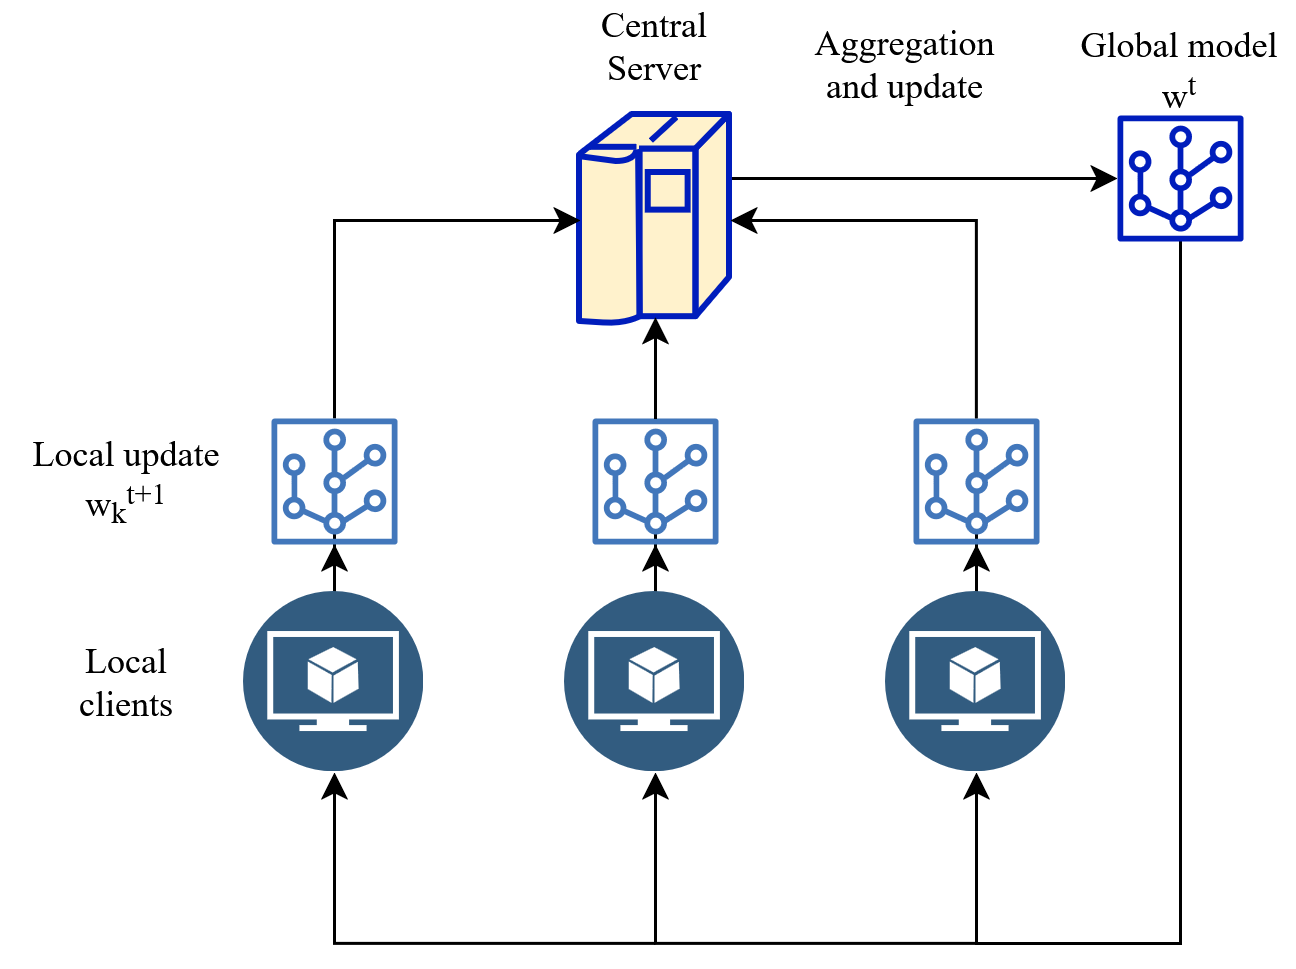
\includegraphics[scale=0.3]{federated_learning.png}
  \caption{Overview of the federated learning pipeline}
  \label{fig:fl-pipeline}
\end{figure}

In each communication round, the server distributes the current global model $w^t$ to a subset of clients. Each selected client initialises its local model with $w^t$ and performs $E$ epochs of stochastic gradient descent on its local data, producing updated parameters $w_k^{t+1}$. The server then aggregates these updates by computing a weighted average:
\begin{equation}
w^{t+1} = \sum_{k=1}^{K} \frac{n_k}{n} w_k^{t+1}
\end{equation}
By performing multiple local training epochs before communication, FedAvg significantly reduces communication costs compared to approaches that require gradient updates after every training step.

Li et al. \cite{liFederatedLearningChallenges2020} surveyed the main challenges. 1) Communication costs are high when bandwidth is limited or models are large. 2) Participating devices vary in compute and connectivity. 3) Data across nodes is usually non-IID. 4) Shared updates can still leak information about training data.

Communication cost is the first of these challenges and has attracted its own line of work. Kone\v{c}n\'y et al. \cite{konecVnyFEDERATEDLEARNINGSTRATEGIES} proposed two ways to reduce communication cost: structured updates, which learn each client update directly in a restricted low-rank or random-mask space, and sketched updates, which compute a full update and then compress it through quantisation, random rotation and subsampling before transmission. Sattler et al. \cite{sattlerRobustCommunicationEfficientFederated2019} observed that earlier compression schemes either ompressed only the client-to-server direction or degraded under non-IID data and proposed sparse ternary compression, which combines top-$k$ sparsification, ternarisation and Golomb encoding of the updates with a mechanism for compressing the downloading as well. Each of these methods trades a small amount of accuracy or convergence speed for a reduction in bytes per round, and the appropriate trade-off depends on the bandwidth available to participating institutions.
\section{Handling Non-IID Data in Federated Learning}

Data distributions across participating nodes are rarely uniform. When each node holds data that is non-IID, local models trained on these subsets may diverge significantly from one another. Averaging such divergent models can produce a global model that performs poorly compared to one trained on centralised data.
 
The mechanism behind this degradation is client drift \cite{karimireddySCAFFOLDStochasticControlled2021}. During the $E$ local epochs of each round, a client's model moves toward the minimiser of its own local objective $F_k$ rather than the global objective $f$. When the local label distribution differs from the global one, these two minimisers are far apart and the local update accumulates a bias in the direction of the local optimum. Drift grows with the number of local steps, the learning rate and the degree of label skew and shrinks when many clients are averaged per round. The methods reviewed below differ in how they act on drift.
 
FedAvg provides no mechanism to limit drift. Li et al. \cite{liFederatedOptimizationHeterogeneous2020} proposed FedProx, which penalises it directly by adding a proximal term to the local objective:
\begin{equation}
\min_{w} h_k(w; w^t) = F_k(w) + \frac{\mu}{2} \| w - w^t \|^2
\end{equation}
where $F_k(w)$ is the local loss, $w^t$ is the current global model and $\mu$ controls the strength of the penalty. The term pulls each local model back toward the global model in proportion to how far it has moved. Its gradient $\mu(w - w^t)$ is zero at the start of local training and grows with drift. This modification provides convergence guarantees under heterogeneous data distributions, which FedAvg lacks. FedProx also accommodates systems heterogeneity by allowing nodes to perform variable amounts of local computation, since a client that completes only part of its local work is still anchored to $w^t$. When $\mu$ is small relative to the local learning rate the penalty is negligible and FedProx reduces to FedAvg; when it is large the penalty dominates the local loss and slows convergence.


Other approaches have been proposed to tackle non-IID issues. Karimireddy et al. \cite{karimireddySCAFFOLDStochasticControlled2021} introduced SCAFFOLD, which uses control variates to correct for the drift in local updates. This reduces the variance caused by heterogeneous data. Wang et al. \cite{wangFederatedLearningMatched2020} proposed Federated Matched Averaging (FedMA), which aligns neurons across local models before averaging. This prevents neurons in different local models from learning equivalent features in different positions. Wang et al. \cite{wangTacklingObjectiveInconsistency2020} proposed FedNova, which normalises local updates to account for differences in the number of local training steps, correcting an inconsistency in FedAvg that is amplified under heterogeneous conditions. While this project focuses on FedAvg and FedProx, these alternative approaches provide context for understanding the breadth of strategies available for handling non-IID data in federated settings.

To evaluate federated learning methods under heterogeneous conditions, a consistent experimental method is required for simulating non-IID data splits. A widely adopted approach, introduced by Hsu et al. \cite{hsuMeasuringEffectsNonIdentical2019}, is to partition data across clients using a Dirichlet distribution over class labels, parameterised by a concentration parameter $\alpha$. Lower values of $\alpha$ produce more skewed label distributions across clients while higher values approach IID. This provides a controllable and reproducible way to study model behaviour across a wide range of heterogeneous conditions.

The theoretical case for drift correction is stronger than evidence suggests. Li et al. \cite{liFederatedLearningNonIID2021} benchmarked FedAvg, FedProx, SCAFFOLD and FedNova on nine datasets under label skew, feature skew and quantity skew partitions and found that no algorithm consistently outperformed the others, with the newer methods beating FedAvg by a clear margin in only a few settings. FedProx tracked FedAvg closely through training in many cases. Having tuned $\mu$ over $\{0.001, 0.01, 0.1, 1\}$, they found the best value was always small, so the proximal term had little effect and the two methods reached similar accuracy at a similar speed. They also found that the number of local epochs had a large effect on accuracy and that its optimal value was sensitive to the partition. Their results suggest that the advantage of a drift-correction method depends on whether the experimental setting produces enough drift for the correction to matter.

\section{Initialisation and Pre-training in Federated Learning}

Most federated learning studies initialise from random weights, whereas centralised image classification almost always starts from weights pre-trained on a large dataset such as ImageNet. Nguyen et al. \cite{nguyenWhereBeginImpact2022} compared the two on four federated benchmarks and found that pre-training reduced the rounds needed to reach a target error, produced models up to 40\% more accurate, and reduced the effect of both data and system heterogeneity; they recommend that federated optimisation methods be evaluated from both initialisations. Chen et al. \cite{chenImportanceApplicabilityPreTraining2023} reached a similar conclusion across several visual recognition benchmarks, with pre-training closing most of the gap between FedAvg and centralised training and giving its largest gains under the most severe non-IID conditions. They attribute this to global models converging to the same loss basin regardless of the client data distribution, which makes aggregation more stable. They note that pre-training does not appear to reduce local drift itself. Instead, what changes is that averaging drifted models still lands in a good region.

This bears directly on method comparison. Drift-correction methods were designed for heterogeneous data and pre-training removes most of the degradation by making aggregation tolerant of drift. Gains reported from random initialisation may therefore not appear when clients fine-tune a shared pre-trained backbone, as is standard in medical imaging.

A second factor specific to convolutional backbones is batch normalisation. ResNet layers carry running statistics estimated from local batches, and Li et al. \cite{liFedBNFederatedLearning2021} showed under feature shift that keeping these layers local and averaging only the remaining parameters (FedBN) outperformed both FedAvg and FedProx.

\section{Privacy in Federated Learning}
Federated learning avoids sharing raw data but this alone does not guarantee privacy. Kaissis et al. \cite{kaissisSecurePrivacypreservingFederated2020} noted that the model updates transmitted during training can be exploited to infer information about the underlying data. Model inversion attacks use model outputs or gradients to reconstruct approximations of training inputs \cite{fredriksonModelInversionAttacks2015}. Membership inference attacks determine whether a specific data point was in the training set by analysing the model's response to that input \cite{shokriMembershipInferenceAttacks2017}.

Several defence mechanisms have been proposed to strengthen privacy in federated learning. Bonawitz et al. \cite{bonawitzPracticalSecureAggregation2017} designed a practical secure aggregation protocol using pairwise masking to protect each participant's contribution. This enables the server to compute the sum of client updates without observing any individual update. This protocol is robust to client dropout, making it suitable for real-world deployments. Differential privacy provides a complementary approach by adding calibrated noise to the data or model updates to limit the information that can be inferred about any individual training example. Dwork et al. \cite{dworkCalibratingNoiseSensitivity2006} established the formal foundations of differential privacy, while Abadi et al. \cite{abadiDeepLearningDifferential2016} introduced DP-SGD, a training procedure that clips per-example gradients and adds noise during optimisation which enables deep learning models to be trained with formal privacy guarantees. These mechanisms can be combined with federated learning to provide stronger privacy protections, though they often introduce trade-offs with model accuracy.

\section{Federated Learning in Medical Imaging}
Federated learning has attracted significant interest in medical imaging, where data is inherently distributed across institutions and subject to strict privacy requirements. Rieke et al. \cite{riekeFutureDigitalHealth2020} outlined the potential of federated learning to enable collaborative model development across hospitals without centralising patient data, identifying it as a key enabler for the future of digital health. They noted that the heterogeneity of clinical data, arising from differences in imaging equipment, protocols, and patient demographics makes the non-IID problem particularly important in this domain.

Sheller et al. \cite{shellerFederatedLearningMedicine2020} demonstrated that federated learning could be applied to brain tumour segmentation across multiple institutions. They achieved performance comparable to centralised training while keeping patient data local. Their work provided early evidence that federated learning is viable in medical imaging tasks with complex, heterogeneous data. More recently, Dayan et al. \cite{dayanFederatedLearningPredicting2021} conducted one of the largest federated learning studies to date, training a model to predict clinical outcomes in COVID-19 patients across 20 institutions worldwide. Their model outperformed any single-institution model, which justifies federated learning in practice.

Federated learning has also been applied to dermatology. The FLamby benchmark \cite{terrailFLambyDatasetsBenchmarks2023} provides seven healthcare datasets with natural client splits for cross-silo federated learning and reports baseline results for several standard strategies, including FedAvg and FedProx, on each. Its dermatology task, Fed-ISIC2019, partitions dermatoscopic images across clients by acquisition centre and classifies eight lesion categories, so the heterogeneity it captures is feature shift arising from real institutional separations. Other work has trained federated classifiers on HAM10000 and ISIC under simulated IID and non-IID splits, typically using FedAvg with a pre-trained CNN backbone. These studies share two features: they use dermatoscopic rather than clinical photographs and they classify fewer than ten lesion categories. None evaluates aggregation methods under controlled label skew on a fine-grained clinical-photograph task.

\section{Summary and Knowledge Gap}
The preceding sections have reviewed the relevant literature across skin disease classification, federated learning, non-IID data handling, privacy mechanisms, and federated learning in medical imaging. Several key gaps emerge from this review:

\begin{enumerate}
  \item \textbf{Limited evaluation of federated learning for multi-class skin disease classification.} Federated learning has been applied successfully in medical imaging but primarily in radiology and pathology tasks with binary or few-class classification. The existing dermatology work uses dermatoscopic lesion datasets with fewer than ten classes. Its performance on fine-grained, multi-class skin disease tasks with 20 or more classes of clinical photographs has not been systematically studied.
  \item \textbf{Insufficient comparison of federated algorithms under realistic non-IID conditions.} While FedProx was designed to address the non-IID limitations of FedAvg, benchmark studies report the two performing similarly, and the pre-training literature predicts that any remaining gap shrinks when clients start from ImageNet weights. Direct comparisons on medical imaging tasks under controlled label skew remain scarce. FLamby compares them on a dermatoscopic task with natural feature-shift splits rather than label skew. Whether a difference appears on a domain-specific dataset where class imbalance and label skew occur is untested.
  \item \textbf{Lack of practical guidance on federated learning trade-offs for clinical imaging.} Existing studies report accuracy but often do not systematically evaluate communication efficiency or per-class performance alongside non-IID sensitivity. Understanding these trade-offs is essential for informing whether federated learning is practical for real-world deployment.
\end{enumerate}

This project addresses these gaps by evaluating FedAvg and FedProx on a 30-class skin disease dataset to simulate realistic data heterogeneity. By comparing these approaches against a centralised baseline on classification accuracy, communication efficiency, and behaviour under non-IID distributions, this project aims to provide practical insight into the suitability of federated learning for fine-grained medical image classification.

\chapter{Methodology}

\section{Project Aims}
Based on the knowledge gaps identified in the preceding chapter, this project has the following aims:
\begin{itemize}
  \item Train a centralised ResNet-18 classifier on a 30-class skin disease dataset of approximately 20,000 clinical photographs to establish an upper-bound benchmark
  \item Run FedAvg and FedProx on the same data, partitioned into IID and Dirichlet non-IID splits across simulated clients
  \item Report how each federated method degrades from the centralised baseline as heterogeneity increases, and what it costs in communication
\end{itemize}

\section{Experimental Pipeline}
The project followed a three-stage pipeline: centralised baseline training, federated training under IID and non-IID partitions and comparative evaluation on a shared held-out test set. All experiments were implemented in Python with PyTorch and run on a single NVIDIA A100 GPU per job.

\subsection{Dataset}
The Massive Skin Disease Balanced Dataset \cite{MassiveSkinDisease} was used as the data source. It is a public Kaggle collection of approximately 262,000 clinical photographs across 34 classes, assembled from several earlier dermatology datasets and balanced by augmenting the smaller classes with flipped, rotated and otherwise transformed copies of their images.

To keep training time manageable across the full experimental grid, a working subset was drawn as follows. The 30 largest classes were retained and 666 images were sampled from each, stratified by the dataset's own train, validation and test assignment so that the split ratio was preserved per class. This produced 19,980 images: 13,980 for training, 3,000 for validation and 3,000 for testing. The test set was held centrally and kept fixed across every experiment. Table~\ref{tab:classes} lists the 30 classes.

\begin{table}[H]
  \centering
  \caption{The 30 classes in the working dataset, 666 images each.}
  \label{tab:classes}
  \small
  \begin{tabular}{ll}
    \hline
    Acne and rosacea & Light diseases and pigmentation disorders \\
    Actinic keratosis, BCC and other malignant lesions & Lupus and other connective tissue diseases \\
    Atopic dermatitis & Malignant \\
    Bacterial: cellulitis & Melanoma, nevi and moles \\
    Bacterial: impetigo & Nail fungus and other nail disease \\
    Bullous disease & Parasitic: cutaneous larva migrans \\
    Cellulitis, impetigo and other bacterial infections & Poison ivy and other contact dermatitis \\
    Exanthems and drug eruptions & Rashes \\
    Fungal: athlete's foot & Scabies, Lyme disease and other infestations \\
    Fungal: nail fungus & Systemic disease \\
    Fungal: ringworm & Urticaria \\
    Hair loss and alopecia & Vascular tumours \\
    Healthy & Vasculitis \\
    Herpes, HPV and other STDs & Viral: chickenpox \\
    Warts, molluscum and other viral infections & Viral: shingles \\
    \hline
  \end{tabular}
\end{table}

Two properties of this dataset require explanation. First, because it merges sources with different labelling schemes, several classes overlap in clinical content. For example, cellulitis and impetigo appear both as single-condition classes and inside a combined bacterial infection class, nail fungus appears twice and the malignant class overlaps with the melanoma and the actinic keratosis classes. Per-class results in Chapters 4 and 5 are examined with this in mind. Second, a large amount of images as augmented copies and the source dataset does not record which original each copy derives from. So an original and its augmentation could in principle fall on different sides of a split. A perceptual-hash check was run over the full 262,874-image split manifest before subsampling, using an 8$\times$8 DCT hash minimised over the eight flip and rotation variants of each image. It found no exact hash collisions, within or across splits. Because the working subset retains each image's original split assignment, that result carries over to it. The check is limited to exact matches under flips and rotations; augmentations involving cropping or colour change, which the \texttt{aug} prefix suggests were used, would not be detected, so some near-duplicate leakage across splits cannot be ruled out.

Images were resized to 256 pixels, randomly cropped to 224, and augmented during training with horizontal flips, colour jitter of 0.1, and rotations of up to 15 degrees, then normalised with ImageNet channel statistics. Validation and test images were resized directly to 224 with no augmentation.

\begin{table}[H]
  \centering
  \caption{Summary statistics of the datasets used in this project.}
  \label{tab:datasets}
  \renewcommand{\arraystretch}{1.3}
  \begin{tabular}{|l|c|c|}
    \hline
    \textbf{Property} & \textbf{Dataset 1} & \textbf{Dataset 2} \\ \hline
    Name & Skin Diseases + Cancer & Massive Skin Disease \\ \hline
    Source & Kaggle & Kaggle \\ \hline
    Total images & $\sim$13,000 & $\sim$262,000 \\ \hline
    Number of classes & 24 & 34 \\ \hline
    Image type & Clinical photographs & Clinical photographs \\ \hline
    Class balance & Imbalanced & Balanced \\ \hline
  \end{tabular}
\end{table}

\subsection{Centralised Baseline}
The training set was partitioned across $K$ simulated clients. In the IID setting the training indices were shuffled and split into $K$ equal shards. In the non-IID setting each class's images were divided among the clients according to proportions drawn from a Dirichlet distribution with concentration $\alpha$ \cite{hsuMeasuringEffectsNonIdentical2019}, with $\alpha \in \{0.1, 0.5, 1.0\}$. Lower $\alpha$ concentrates each class on fewer clients. Clients left with fewer than two images were dropped, which did not occur in any run. Table~\ref{tab:partition} summarises the partitions produced with $K = 10$ and seed 42.

\begin{table}[H]
  \centering
  \caption{Partition statistics for $K = 10$ clients, seed 42. Empty class cells counts client--class pairs with no images, out of $10 \times 30$.}
  \label{tab:partition}
  \begin{tabular}{lccc}
    \hline
    Partition & Client size (min--max) & Classes per client (min--max) & Empty class cells \\ \hline
    IID & 1,398--1,398 & 30--30 & 0/300 \\
    $\alpha = 1.0$ & 1,028--1,738 & 29--30 & 2/300 \\
    $\alpha = 0.5$ & 659--1,843 & 26--30 & 17/300 \\
    $\alpha = 0.1$ & 288--3,667 & 8--27 & 136/300 \\ \hline
  \end{tabular}
\end{table}

The three $\alpha$ values span a wide range of heterogeneity. At $\alpha = 1.0$ and $\alpha = 0.5$ every client still holds at least 26 of the 30 classes and client sizes vary by less than a factor of three, so these partitions differ from IID mainly in class proportions rather than class presence. At $\alpha = 0.1$ the largest client holds nearly 13 times as many images as the smallest, clients see between 8 and 27 classes, and 45\% of client--class pairs are empty, so most clients never encounter most classes during local training. This is the only partition in which label skew is severe, and it is where the methods are expected to separate if they separate at all.

\subsection{Evaluation}

All models were evaluated on the same 3,000-image test set using the following metrics.

\begin{itemize}
  \item \textbf{Classification accuracy}: overall test accuracy.
  \item \textbf{Per-class performance}: precision, recall and F1-score per class, with macro-averaged F1 as the summary. This is reported because the class set contains clinically overlapping categories whose confusion is not visible in overall accuracy.
  \item \textbf{Communication cost}: the total volume of parameter data transmitted, counting the full model state (11.19 million parameters plus BatchNorm buffers, 44.81 MB) once from server to client and once back for every participating client in every round, and the number of rounds required for validation accuracy to reach 0.85, computed after training from the per-round logs at two-round resolution.
  \item \textbf{Non-IID sensitivity}: test accuracy as a function of $\alpha$ for each method.
\end{itemize}
Results for FedAvg and FedProx are compared against each other and against the centralised baseline, as mean and standard deviation over seeds.

\section{Ethical Considerations}
This project used a single publicly available skin disease image dataset obtained from Kaggle. The dataset was released by its author for research and educational purposes and contains no directly identifying patient information such as names or dates of birth. No new patient data was collected, and no human or animal subjects were involved in the research. For these reasons, formal ethics approval was not required for this project.

Several ethical considerations remained relevant. Publicly released medical image datasets may still carry risks of re-identification. All data was treated as sensitive and no attempt was made to link images back to individuals or external sources.

Skin disease classifiers are known to exhibit performance disparities across skin tones, as publicly available datasets are often skewed toward lighter skin types. Results are interpreted with this limitation in mind, and per-class performance metrics are reported to surface any systematic disparities.

While this project was a simulation and did not involve clinical deployment, the broader motivation carries downstream implications for patient privacy, model accountability, and the trustworthiness of clinical AI systems. This project is a methodological evaluation and no diagnostic claims follow from it.

All code, experimental configurations, and results were managed with version control to support reproducibility, and the dataset is cited so that others can verify and build upon the work.

\chapter{Study 1: Centralised Baseline and IID Federated Learning}

\section{Aims}
This study establishes the two reference points for the rest of the thesis. The centralised baseline sets the accuracy ceiling for the architecture and dataset. The IID federated runs test whether FedAvg and FedProx reach that ceiling when every client holds a representative sample of the data. An IID partition produces no systematic client drift, so FedProx should match FedAvg here, which makes this study a consistency check on the FedProx implementation as well.

\section{Methods}
The baseline was trained as described in Section 3.2.2. FedAvg and FedProx ($\mu = 0.001$) were run under the IID partition with $K = 10$, $C = 0.5$, $E = 5$ and $B = 32$ for 100 rounds, with seeds 42, 43 and 44. All three models were evaluated on the shared 3,000-image test set.

\section{Results}
\subsection{Centralised baseline}
The baseline reached a test accuracy of 0.877 and macro F1 of 0.875, with the best validation checkpoint at epoch 24 of 25. The baseline was trained once, with seed 42. Table~\ref{tab:baseline-perclass} gives per-class F1 for the ten weakest and ten strongest classes. The five weakest classes are broad umbrella categories that each group several conditions: Warts Molluscum and Other Viral Infections (F1 0.600), Systemic Disease (0.681), Light Diseases and Disorders of Pigmentation (0.727), Actinic Keratosis Basal Cell Carcinoma and Other Malignant Lesions (0.765) and Lupus and Other Connective Tissue Diseases (0.766). The strongest classes are narrow single conditions, including Nail Fungus and Shingles (1.000), Athlete's Foot and Chickenpox (0.995) and Cutaneous Larva Migrans (0.990). With one exception, these are not the overlapping classes identified in Section 3.2.1: only the actinic keratosis class overlaps with another (Malignant), while the remaining four weakest classes are umbrella categories with no equivalent elsewhere in the label set. The overlapping classes themselves were separable. Nail Fungus reached F1 of 1.000 despite the presence of a second nail disease class. The most likely explanation is that overlapping classes come from different source datasets within the Kaggle collection, whose photographic style differs. This means the model can separate them on source rather than on clinical content. This is a limitation of the dataset rather than a strength of the classifier and per-class results for these classes should not be treated as evidence that the model distinguishes these.

\begin{table}[H]
  \centering
  \caption{Per-class test F1 for the centralised baseline, ten lowest and ten highest, sorted ascending. Every class has 100 test images.}
  \label{tab:baseline-perclass}
  \small
  \begin{tabular}{p{9cm}ccc}
  \hline
  Class & Precision & Recall & F1 \\ \hline
  Warts, Molluscum and Other Viral Infections & 0.675 & 0.540 & 0.600 \\
  Systemic Disease & 0.727 & 0.640 & 0.681 \\
  Light Diseases and Disorders of Pigmentation & 0.735 & 0.720 & 0.727 \\
  Actinic Keratosis, BCC and Other Malignant Lesions & 0.781 & 0.750 & 0.765 \\
  Lupus and Other Connective Tissue Diseases & 0.734 & 0.800 & 0.766 \\
  Exanthems and Drug Eruptions & 0.789 & 0.750 & 0.769 \\
  Vascular Tumors & 0.777 & 0.800 & 0.788 \\
  Herpes, HPV and Other STDs & 0.773 & 0.850 & 0.810 \\
  Scabies, Lyme Disease and Other Infestations and Bites & 0.790 & 0.830 & 0.810 \\
  Atopic Dermatitis & 0.825 & 0.850 & 0.837 \\
  \multicolumn{4}{c}{$\cdots$} \\
  Malignant & 1.000 & 0.950 & 0.974 \\
  Bacterial: Cellulitis & 0.961 & 0.990 & 0.975 \\
  Healthy & 0.962 & 1.000 & 0.980 \\
  Bacterial: Impetigo & 0.980 & 1.000 & 0.990 \\
  Fungal: Ringworm & 0.980 & 1.000 & 0.990 \\
  Parasitic: Cutaneous Larva Migrans & 0.980 & 1.000 & 0.990 \\
  Fungal: Athlete's Foot & 0.990 & 1.000 & 0.995 \\
  Viral: Chickenpox & 0.990 & 1.000 & 0.995 \\
  Fungal: Nail Fungus & 1.000 & 1.000 & 1.000 \\
  Viral: Shingles & 1.000 & 1.000 & 1.000 \\
  \hline
\end{tabular}
\end{table}

\subsection{IID federated learning}
Table~\ref{tab:iid} reports FedAvg and FedProx under the IID partition. FedAvg reached 0.875 $\pm$ 0.001 test accuracy, 0.2 points below the centralised baseline. FedProx reached 0.873 $\pm$ 0.002, 0.4 points below the baseline; paired by seed, it matched FedAvg on one seed and was lower by 0.14 and 0.20 points on the other two (mean difference $-0.11 \pm 0.10$ points). Figure~\ref{fig:iid-curves} shows validation accuracy by round. Both methods passed 0.85 validation accuracy by round 22, FedAvg after 19.3 $\pm$ 1.2 rounds and FedProx after 20.0 $\pm$ 2.0, and both plateaued, defined as reaching within 0.5 points of the peak seed-mean validation accuracy, by round 36. The best checkpoint occurred between rounds 60 and 74 for FedAvg and between rounds 48 and 88 for FedProx.

\begin{table}[H]
  \centering
  \caption{Test performance under IID partitioning, mean $\pm$ std over three seeds. Rounds to 0.85 is measured on validation accuracy.}
  \label{tab:iid}
  \begin{tabular}{lcccc}
    \hline
    Method & Accuracy & Macro F1 & Rounds to 0.85 & Communication (GB) \\ \hline
    Centralised & 0.877 & 0.875 & -- & -- \\
    FedAvg & 0.875 $\pm$ 0.001 & 0.873 $\pm$ 0.001 & 19.3 $\pm$ 1.2 & 44.8 \\
    FedProx ($\mu = 0.001$) & 0.873 $\pm$ 0.002 & 0.872 $\pm$ 0.002 & 20.0 $\pm$ 2.0 & 44.8 \\ \hline
  \end{tabular}
\end{table}

\begin{figure}[H]
  \centering
  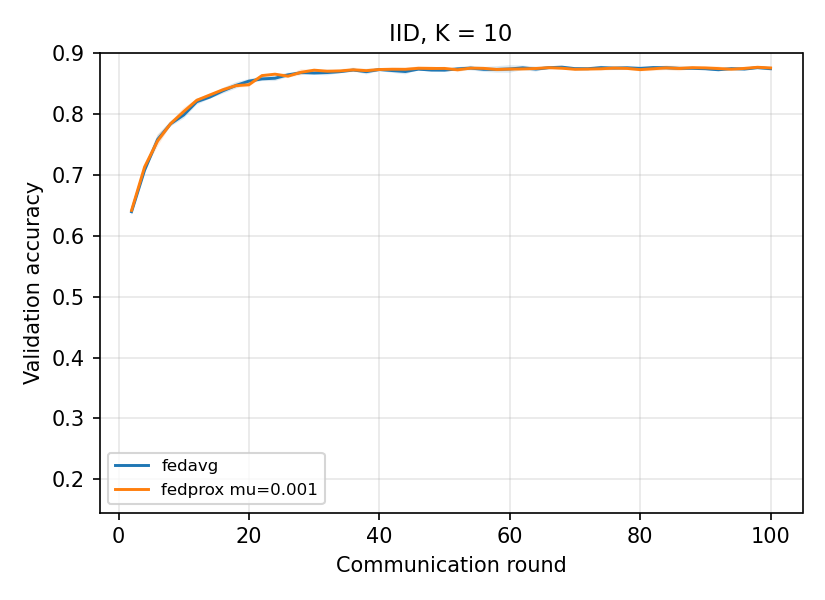
\includegraphics[width=0.7\linewidth]{curves_iid_c10.png}
  \caption{Validation accuracy per communication round under IID partitioning}
  \label{fig:iid-curves}
\end{figure}

\section{Discussion}
Under IID partitioning, federated training recovered the centralised baseline to within seed variation. FedAvg's 0.2-point gap and FedProx's 0.4-point gap are of the same order as the spread across seed, and the paired difference between the two methods ($-0.11 \pm 0.10$ points) is not distinguishable from zero with three seeds. This is consistent with Sheller et al. \cite{shellerFederatedLearningMedicine2020}, who reported federated models reaching 99\% of centralised quality on homogeneous institutional data. The cost of federation in this setting is communication alone: reaching 0.85 validation accuracy took about 20 rounds and 9 GB of transfer and the full 100-round budget cost 44.8 GB.

FedAvg and FedProx were indistinguishable, as expected. With representative client data the local minimisers coincide with the global one, so the proximal gradient $\mu(w - w^t)$ stays near zero throughout local training and FedProx reduces to FedAvg. This confirms that the implementation adds no overhead or bias at small $\mu$, so any separation between the methods in Chapter 5 can be attributed to heterogeneity rather than to the methods' behaviour on homogeneous data.

Two features of the IID curves carry forward. Both methods reached within 0.5 points of their peak by round 36 and then improved slowly, so the 100-round budget was generous for this partition. The best checkpoint nonetheless fell in the second half of training for every seed, so the late improvement show is real instead of just noise. Chapter 5 examines how both features change as $\alpha$ decreases.

The per-class results constrain what the test set can measure. Because the strongest and weakest classes separate cleanly by source collection, overall accuracy on this dataset is partly a measure of how well a model identifies image provenance and the classes with near-perfect F1 contribute a fixed ceiling that every method reaches. The comparisons in Chapter 5 are unaffected, since every method is scored on the same images, but the absolute accuracies reported in this thesis should not be read as estimates of clinical diagnostic performance. The baseline was trained with a single seed, so its 0.877 carries no error bar. The federated IID spread of 0.001 to 0.002 suggests the baseline's own seed variation is of similar size.

\chapter{Study 2: Federated Learning under Non-IID Conditions}

\section{Aims}
\begin{itemize}
  \item Evaluate how FedAvg and FedProx degrade as data heterogeneity increases.
  \item Assess whether the FedProx proximal term improves stability and accuracy under label skew.
\end{itemize}

\section{Methods}
\begin{itemize}
  \item Dirichlet partitioning with $\alpha \in \{0.1, 0.5, 1.0\}$.
  \item FedProx proximal weight tuned over $\mu \in \{0.001, 0.01, 0.1, 1.0\}$.
\end{itemize}

\section{Results}
\begin{itemize}
  \item To be completed: accuracy as a function of $\alpha$ for both methods.
  \item To be completed: communication rounds to target accuracy, per-class performance on minority classes.
\end{itemize}

\section{Discussion}
\begin{itemize}
  \item To be completed: comparison of FedAvg and FedProx degradation, practical implications for federated medical imaging.
\end{itemize}

\chapter{General Discussion and Conclusions}
\section{Summary}
\begin{itemize}
  \item To be completed: summary of baseline, IID, and non-IID findings.
\end{itemize}
\section{Discussion and Future Work}
\begin{itemize}
  \item To be completed: how the two studies together answer the project aims.
  \item Planned future directions: stronger architectures such as Vision Transformers, non-IID improvements, communication optimisations.
\end{itemize}
\section{Conclusions}
\begin{itemize}
  \item To be completed: overall assessment of whether federated learning is a viable substitute for centralised training in this setting, and under what heterogeneity conditions.
\end{itemize}

\cleardoublepage

\addcontentsline{toc}{chapter}{Bibliography}
\bibliographystyle{unsrtnat}
\bibliography{references}

\appendix

\newpage
\addcontentsline{toc}{part}{Appendices}
\mbox{}
\newpage

\chapter{Program listings}
Code and experimental configurations will be made available via a GitHub repository, with directions provided in the final thesis.

\end{document}